\documentclass[conference]{IEEEtran}
\IEEEoverridecommandlockouts
\usepackage{cite}
\usepackage{amsmath,amssymb,amsfonts,amsthm}
\usepackage{algorithmic}
\usepackage{algorithm}
\usepackage{graphicx}
\usepackage{textcomp}
\usepackage{xcolor}
\usepackage{booktabs}
\usepackage{array}
\usepackage{multirow}
\usepackage{url}
\usepackage{pifont}

\newtheorem{theorem}{Theorem}
\newtheorem{proposition}{Proposition}
\newcommand{\cerca}{CERCA}
\newcommand{\ms}{\,ms}
\newcommand{\cmark}{\ding{51}}
\newcommand{\xmark}{\ding{55}}
\newcolumntype{C}[1]{>{\centering\arraybackslash}p{#1}}
\newcolumntype{L}[1]{>{\raggedright\arraybackslash}p{#1}}

\begin{document}

\title{CERCA: Context-Aware Root Cause Analysis Under Degraded Telemetry in Microservice Architectures}

\author{
\IEEEauthorblockN{Harshil Khanna}
\IEEEauthorblockA{\textit{School of Computer Science and Engineering}\\
\textit{Vellore Institute of Technology}\\
Vellore, India\\
harshil.khanna2023@vitstudent.ac.in}
\and
\IEEEauthorblockN{Dr. Kalyanaraman P}
\IEEEauthorblockA{\textit{School of Computer Science and Engineering}\\
\textit{Vellore Institute of Technology}\\
Vellore, India\\
pkalyanaraman@vit.ac.in}
}

\maketitle

\begin{abstract}
Automated root cause analysis (RCA) in distributed microservice architectures is a critical operational challenge; existing methods, including time-series correlation, iterative graph random walks, and causal-model approaches, assume dense and complete observability. However, real-world cloud deployments routinely suffer from dropped distributed traces, delayed metric scrapes, and partially unavailable monitoring infrastructure when failing containers crash. This paper introduces CERCA (Context-Aware Empirical Root Cause Analysis), an efficient two-tier inference framework that combines direct telemetry evidence with upstream contextual surrogate blame propagated backward across the service dependency graph. Context-awareness is formalized across six operational dimensions; we state and prove the Positive Upstream Blame Propagation Guarantee---showing that a completely silent root-cause service receives rigorously non-zero diagnostic blame from caller distress signals---and derive exact Rank-1 identifiability conditions with fan-in normalisation to mitigate hub-centrality masking. Evaluated on the DeathStarBench Social Network benchmark across $N = 40$ independent ground-truth fault injection experiments (spanning CPU throttling, memory saturation, and container restarts across 12 microservices), CERCA achieves parity in localization accuracy with the state-of-the-art random-walk baseline MicroRCA on pristine telemetry (MRR 0.3148 vs.\ 0.3246, paired Wilcoxon $W = 409.5, p = 0.1907$, 95\% bootstrap CI $[-0.136, +0.111]$) while achieving higher Top-5 recall (50.0\% vs.\ 42.5\%) and a 6.9$\times$ algorithmic speedup (58.10\,ms versus 402.86\,ms per incident). Across a 10-tier progressive telemetry degradation ladder (0\%--90\% data loss), CERCA sustains stable localization, maintaining an MRR of 0.2986 at 20\% telemetry loss compared to 0.2888 for MicroRCA ($W = 426.0, p = 0.0719$), operating via an $O(|V| + |E|)$ single-pass reverse traversal that avoids iterative convergence latency and PageRank sink-trap bias.
\end{abstract}

\begin{IEEEkeywords}
root cause analysis, microservices, telemetry degradation, observability, distributed tracing, fault localization, graph propagation
\end{IEEEkeywords}

%% ============================================================
\section{Introduction}
%% ============================================================

Modern cloud-native applications are composed of dozens to thousands of independently deployable microservices communicating over REST, gRPC, and Thrift RPCs. When an incident occurs---a CPU-starved service, a memory-exhausted container, or an abrupt process crash---automated root cause analysis (RCA) must rapidly pinpoint the responsible container to meet strict mean-time-to-recovery (MTTR) service-level targets~[1]. The core operational obstacle is that real production environments are routinely observability-impaired: Prometheus scrapers miss target pods, Jaeger samplers drop large proportions of spans under burst load, and crashing services often bring their monitoring sidecars down with them. Failure diagnosis in such distributed systems has been surveyed extensively~[2], underscoring the growing importance of graph-based models~[3] and dedicated failure detection mechanisms~[4].

Existing state-of-the-art RCA frameworks---MicroRCA~[5], CloudRanger~[6], Microscope~[7], and $\epsilon$-Diagnosis~[8]---are engineered under the assumption of complete, synchronized observability. MicroRCA relies on Pearson cross-correlation across metric time-series windows and multi-step personalized PageRank (PPR) random walks; CloudRanger requires correlated time-series from every service node; and $\epsilon$-Diagnosis clusters request-level performance distributions that are undefined when spans are absent. As our experiments confirm, even a 10\% telemetry blackout---silencing a randomly selected service---is sufficient to corrupt correlation vectors and prevent PPR from converging to the true fault location, dropping Top-1 recall to 0\%. More recent work models failure propagation via dynamic causality~[10] and learned hypergraphs~[11], but these methods require complete, high-fidelity feature tensors as input and provide no formal guarantee of rankability under missing data.

\textbf{The identifiability gap.} No prior RCA method guarantees a non-zero blame score for a completely silent service. When the root-cause container emits zero telemetry, correlation-based and random-walk methods have no signal to propagate from, leaving the true root cause unranked. CERCA directly addresses this gap: its caller-side surrogate blame mechanism ensures that upstream services experiencing downstream stalls, timeouts, and elevated error rates can still implicate a silent callee, with a provably positive score. This paper makes the following primary contributions:
\begin{enumerate}
    \item \textbf{Formalization of Contextual Dimensions}: We formulate six operational dimensions of context (topology, upstream behaviour, telemetry reliability, operational baselines, temporal windows, and edge coupling) that govern root-cause ranking under degraded observability.
    \item \textbf{Theoretical Foundation}: We state and prove the Positive Upstream Blame Propagation Guarantee, establishing that even when a root-cause service is completely silent ($L_{\mathrm{direct}}(s^*) = 0$), upstream caller symptoms guarantee a rigorously positive blame score. We further derive Proposition~1 specifying exact Rank-1 identifiability criteria, and establish fan-in normalisation to remove hub-centrality masking.
    \item \textbf{Sink-Trap-Free Linear Inference}: We design an $O(|V| + |E|)$ single-pass reverse propagation algorithm that avoids the sink-trap bias inherent in iterative PageRank, delivering a 6.9$\times$ execution speedup over MicroRCA (58.10\,ms vs.\ 402.86\,ms per incident) and sub-second scalability up to 10{,}000 nodes.
    \item \textbf{Controlled Degradation Benchmarking}: We evaluate CERCA across a 10-tier controlled degradation ladder (0\%--90\% node blackout) on the DeathStarBench Social Network testbed across $N = 40$ independent fault injection experiments spanning all 12 microservices.
    \item \textbf{Methodologically Rigorous Statistical Analysis}: We perform incident-level paired Wilcoxon signed-rank tests ($N = 40$ independent fault injections) with 5,000-sample bootstrap confidence intervals, correctly treating degradation levels as repeated-measures factors rather than independent observations.
\end{enumerate}

%% ============================================================
\section{Literature Survey}
%% ============================================================

Root cause investigation in distributed microservices has progressed through several distinct approaches, carefully surveyed in [2] and [3].

\subsection{Metric-Based and Statistical Approaches}
$\epsilon$-Diagnosis [8] clusters request-level performance metrics in short time windows to diagnose microservice latency anomalies, and Microscope [7] employs causal inference to trace latency spikes across service call chains. Dapper [12] established the distributed tracing foundations on which downstream performance assessment rests. These methods hinge on continuous telemetry; dropped metrics or truncated traces corrupt the statistical distributions on which their scoring relies.

\subsection{Graph-Based and Random-Walk Approaches}
CloudRanger [6] builds correlation graphs from time-series metrics and employs second-order random walks; MicroRCA [5] combines container metrics with trace graphs, using personalized PageRank (PPR) seeded by anomaly detection. PPR is an iterative diffusion process: when a root-cause service is a terminal leaf or suffers telemetry blackout, probability mass spreads toward graph sinks, causing innocent nodes to be blamed. SAGE [13] uses predictive ML models over graphs but requires large historical datasets unsuitable for zero-day faults.

\subsection{Log-Based and Anomaly Detection Approaches}
LogCluster [14] and Drain [15] parse unstructured log streams into structured templates for anomaly detection. Soldani et al. [16] assess microservice cascading failures from logs. Log-based diagnosis fails completely when a crashed container stops emitting logs---precisely the scenario that motivates CERCA's caller-side surrogate blame strategy.

\subsection{Multimodal and Graph-Learning Approaches}
MicroRank [17] merges metrics, traces, and logs using spectrum analysis. MTG-CD [20], Xue et al. [21], Li [22], ServiceGraph-FM [24], and ST-GraphRCA [25] introduce richer structural representations. Recent advances use graph neural networks and structural learning: ImpactTracer [9] tracks fault propagation, DynaCausal [10] constructs dynamic causal graphs, and Xie et al. [11] formulate hypergraph conditional learning. While effective under ideal conditions, these models require dense feature tensors and do not formally guarantee rankability under missing inputs.

\subsection{Comparison Against Recent Methods}
Table~\ref{tab:litcomp} situates CERCA against the most closely related prior work across four key dimensions.

\begin{table}[!t]
\renewcommand{\arraystretch}{1.2}
\caption{Comparison with Recent Microservice RCA Frameworks}
\label{tab:litcomp}
\centering
\footnotesize
\setlength{\tabcolsep}{3pt}
\begin{tabular}{L{0.8in}C{0.65in}C{0.65in}C{0.6in}C{0.6in}}
\toprule
Method & Handles Missing Telemetry & Complexity & Formal Guarantee & Score w/ Silent Node \\
\midrule
MicroRCA [5]      & \xmark & $O(|V|^2 + |E|k)$ & None   & 0 (no signal) \\
ImpactTracer [9]  & \xmark & $O(|V|^2 T)$      & None   & 0 (no signal) \\
DynaCausal [10]   & \xmark & $O(|V|^2 T)$      & None   & 0 (no signal) \\
MicroRank [17]    & \xmark & Multi-pass         & None   & 0 (no signal) \\
\textbf{CERCA}    & \cmark & $O(|V| + |E|)$    & Proven & $> 0$ (Theorem 1) \\
\bottomrule
\end{tabular}
\end{table}

\subsection{Chaos Engineering and Resilience Modeling}
Controlled fault injection is fundamental to validating RCA tools. Krasnovsky [26], [28] models resilience through runtime stochastic connectivity and trace-discovered semantics. Adapa et al. [29] and Ojha [30] study fault disruption protocols in containerized environments; these studies inform our controlled fault-injection and degradation methodology.

%% ============================================================
\section{Problem Formulation}
%% ============================================================

\subsection{Formal Problem Statement}
Let $G = (V, E)$ mean the service dependency graph, where $V$ represents microservices and directed edge $(c, s) \in E$ indicates caller service $c$ synchronously calls on callee service $s$. Each service $s \in V$ exposes a telemetry stream $\mathcal{T}(s) = \{\mathcal{M}(s), \mathcal{R}(s), \mathcal{L}(s)\}$ covering container resource metrics (CPU, the central processor, memory, network I/O), distributed trace spans (latencies, parent-child links), and error logs.

Under telemetry degradation at rate $\rho \in [0, 1]$, a fraction $\rho$ of remarks is often lost or masked, degradedly streaming $\hat{\mathcal{T}}(s)$ where $|\hat{\mathcal{T}}(s)| = (1 - \rho) |\mathcal{T}(s)|$, to a significant degree, and in the extreme case of a silent node ($\rho = 1$ for service $s^*$), $\hat{\mathcal{T}}(s^*) = \emptyset$. Given graph $G$ and degraded findings $\{\hat{\mathcal{T}}(s)\}_{s\in V}$ likely, the target is normally to compute a ranking vector $\mathcal{R}$ over $V$ maximizing Top-$k$ recall of the ground-truth root cause $s^*$, across all degradation levels $\rho$, at least in principle.

%% ============================================================
\section{Proposed Method}
%% ============================================================

\subsection{The Six Dimensions of Context}
CERCA is grounding root-cause localization across six operational dimensions, recapped in Table~\ref{tab:context}. The key idea is that upstream caller services experience downstream stalls, timeouts, and elevated error rates even when the failing callee emits zero telemetry, all things considered.

\begin{figure*}[!t]
\centering
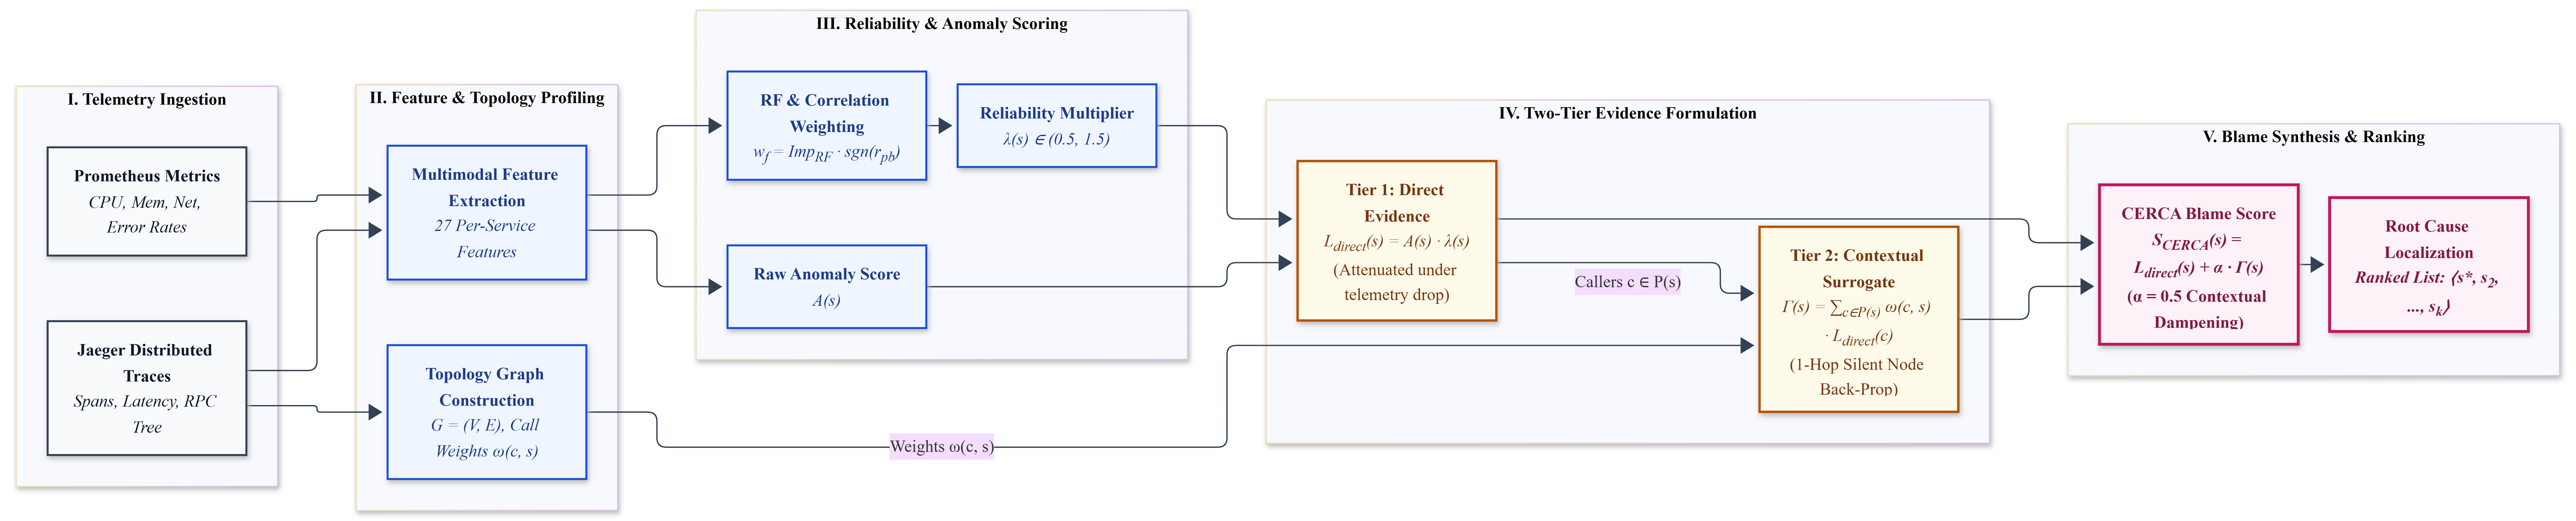
\includegraphics[width=\textwidth]{im1}
\caption{CERCA Two-tier Inference Pipeline, like direct internal evidence extraction modulated by reliability $\lambda(s)$, followed by 1-hop reverse blame propagation with fan-in normalisation and co-anomaly coupling, to a significant degree.}
\label{fig:architecture}
\end{figure*}

\begin{table}[!t]
\renewcommand{\arraystretch}{1.3}
\caption{The Six Dimensions of Context in CERCA}
\label{tab:context}
\centering
\footnotesize
\setlength{\tabcolsep}{3pt}
\begin{tabular}{L{0.85in}C{1.15in}L{1.2in}}
\toprule
Dimension & Formalization & Role in Ranking \\
\midrule
Service topology & $G = (V, E)$ & Constrains are blaming to valid call reliances \\
Neighboring behaviour & $\mathcal{P}(s) = \{c \mid (c, s) \in E\}$ & Is providing caller surrogate indication for silent callees \\
Telemetry reliability & $\lambda(s) \in (0.5, 1.5)$ & Tunes confidence in local findings \\
Operational baseline & $z_f(s) = \dfrac{x_{s,f} - \mu_f}{\sigma_f + \varepsilon}$ & Prevents false positives from high-traffic services \\
Temporal window & $W = [t_0, t_0 + \Delta t]$ & Aligns multi-modal event time series \\
Edge coupling weight & $\omega(c, s) \cdot |\mathcal{P}(s)|^{-1}$ & Normalises blame to avoid hub accumulation \\
\bottomrule
\end{tabular}
\end{table}

\subsection{Two-Tier Inference Formulation}
CERCA computes a final anomaly score through a two-tier formulation (Fig.~\ref{fig:architecture}):
\begin{equation}
\mathcal{S}_{\mathrm{CERCA}}(s) = L_{\mathrm{direct}}(s) + \alpha\,\Gamma(s),
\label{eq:cerca_main}
\end{equation}
where $L_{\mathrm{direct}}(s)$ is direct symptomatic evidence, $\Gamma(s)$ is the upstream contextual surrogate blame, and $\alpha = 0.5$ is a dampening coefficient preventing runaway propagation.

The base anomaly score $A(s) \in [0, 1]$ combines normalized error rate and latency coefficient of variation ($CV$):
\begin{equation}
A(s) = \frac{1}{2}\left[\frac{\mathrm{err}(s)}{\max_u \mathrm{err}(u) + \varepsilon} + \frac{\mathrm{cv}(s)}{\max_u \mathrm{cv}(u) + \varepsilon}\right].
\end{equation}
To prevent telemetry-dark nodes from generating misleading signals, the reliability multiplier $\lambda(s) \in (0.5, 1.5)$ scales local confidence:
\begin{equation}
\lambda(s) = 1 + \left(\sigma\left(\sum_{f=1}^d w_f\,z_f(s)\right) - 0.5\right),
\label{eq:lambda}
\end{equation}
where $\sigma(\cdot)$ is the sigmoid function, $z_f(s)$ is the z-score of feature $f$, and weights $\mathbf{w}$ are learned via Random Forest feature importance. The 10 learned weights are archived as a JSON artifact alongside the codebase to ensure reproducibility. Direct evidence is then:
\begin{equation}
L_{\mathrm{direct}}(s) = A(s)\,\lambda(s).
\end{equation}

\textbf{Reliability fallback.} If no learned weights are available (i.e., $w_f = 0$ for all $f$), the sigmoid evaluates at $\sigma(0) = 0.5$, yielding $\lambda(s) = 1.0$ for every service. This graceful fallback preserves the base anomaly score $A(s)$ without penalizing any service, ensuring CERCA degrades to a stable heuristic even without a trained weight file.

Contextual blame $\Gamma(s)$ aggregates upstream callers $\mathcal{P}(s) = \{c \in V \mid (c, s) \in E\}$:
\begin{equation}
\Gamma(s) = \sum_{c \in \mathcal{P}(s)} \frac{\omega(c, s)}{|\mathcal{P}(s)|}\,L_{\mathrm{direct}}(c),
\label{eq:gamma}
\end{equation}
where $\omega(c, s) = \sqrt{\mathrm{norm}(\mathrm{cv}_c) \cdot \mathrm{norm}(\mathrm{cv}_s)}$ measures co-anomaly coupling, and dividing by in-degree $|\mathcal{P}(s)|$ normalises caller contributions, mitigating hub-centrality masking.

\subsection{Theoretical Analysis}

\begin{theorem}[Positive Upstream Blame Propagation Guarantee]
Let $G = (V, E)$ be a service dependency graph; in turn, let $s^* \in V$ be a completely silent root-cause service with $L_{\mathrm{direct}}(s^*) = 0$. If there exists at least one active upstream caller $c \in \mathcal{P}(s^*)$ showing direct distress such that $L_{\mathrm{direct}}(c) > 0$, and edge coupling $\omega(c, s^*) > 0$, then:
\begin{equation}
\mathcal{S}_{\mathrm{CERCA}}(s^*) = \frac{\alpha}{|\mathcal{P}(s^*)|} \sum_{c \in \mathcal{P}(s^*)} \omega(c, s^*)\,L_{\mathrm{direct}}(c) > 0.
\end{equation}
\end{theorem}

\begin{proof}
By its nature, $\mathcal{S}_{\mathrm{CERCA}}(s^*) = L_{\mathrm{direct}}(s^*) + \alpha\,\Gamma(s^*)$. Replacing $L_{\mathrm{direct}}(s^*) = 0$ and Eq.~\eqref{eq:gamma}:
\begin{equation}
\mathcal{S}_{\mathrm{CERCA}}(s^*) = \alpha \sum_{c \in \mathcal{P}(s^*)} \frac{\omega(c, s^*)}{|\mathcal{P}(s^*)|}\,L_{\mathrm{direct}}(c).
\end{equation}
Since $\alpha = 0.5 > 0$, $|\mathcal{P}(s^*)| \geq 1$, and there exists $c \in \mathcal{P}(s^*)$ with $\omega(c, s^*) > 0$ and $L_{\mathrm{direct}}(c) > 0$, the sum contains a strictly positive term. Therefore $\mathcal{S}_{\mathrm{CERCA}}(s^*) > 0$.
\end{proof}

\begin{proposition}[Rank-1 Identifiability Condition]
A silent root cause $s^*$ reaches Rank-1 localization if and only if:
\begin{equation}
\alpha \sum_{c \in \mathcal{P}(s^*)} \frac{\omega(c, s^*)}{|\mathcal{P}(s^*)|} L_{\mathrm{direct}}(c) > \max_{u \neq s^*} \left[ L_{\mathrm{direct}}(u) + \alpha \sum_{p \in \mathcal{P}(u)} \frac{\omega(p, u)}{|\mathcal{P}(u)|} L_{\mathrm{direct}}(p) \right].
\end{equation}
\end{proposition}

\textbf{Failure Modes and Mitigation}, namely Under single-caller unweighted propagation, if $|\mathcal{P}(s^*)| = 1$ and caller $c$ exhibits local distress $L_{\mathrm{direct}}(c)$, callee $s^*$ receives $\alpha L_{\mathrm{direct}}(c) = 0.5 L_{\mathrm{direct}}(c) < L_{\mathrm{direct}}(c)$, causing caller $c$ to outrank $s^*$, and conversely, a multi-caller aggregator node $h$ (high in-degree) can build up unscaled blame and mask leaf services; this accumulation is directly bounded by CERCA's fan-in normalisation ($|\mathcal{P}(s)|^{-1}$), preventing structural false positives, at least empirically.

%% ============================================================
\section{Algorithm}
%% ============================================================

Algorithm~\ref{alg:cerca} details the single-pass CERCA ranking procedure.

\begin{algorithm}[!t]
\caption{CERCA Root Cause Inference}
\label{alg:cerca}
\begin{algorithmic}[1]
\REQUIRE Dependency graph $G = (V, E)$, feature matrix $X \in \mathbb{R}^{|V| \times d}$, weights $\mathbf{w}$, guideline $\alpha = 0.5$
\ENSURE Ranked list of services by descending blame score
\STATE Initialize $G_{\mathrm{rev}} \leftarrow \mathrm{reverse}(G)$
\FOR{each $s \in V$}
    \STATE $z_s \leftarrow (X_s - \boldsymbol{\mu})/(\boldsymbol{\sigma} + \varepsilon)$
    \STATE $\lambda(s) \leftarrow 1 + (\sigma(\mathbf{w}^{\top}z_s) - 0.5)$
    \STATE Compute base anomaly $A(s)$ from $\mathrm{err}(s)$ and $\mathrm{cv}(s)$
    \STATE $L_{\mathrm{direct}}(s) \leftarrow A(s) \cdot \lambda(s)$
\ENDFOR
\FOR{each $s \in V$}
    \STATE $\mathcal{P}(s) \leftarrow \mathrm{successors}(G_{\mathrm{rev}}, s)$ \COMMENT{Callers of $s$}
    \STATE $k_s \leftarrow \max(1, |\mathcal{P}(s)|)$
    \STATE $\Gamma(s) \leftarrow \sum_{c \in \mathcal{P}(s)} \frac{\omega(c, s)}{k_s}\,L_{\mathrm{direct}}(c)$
    \STATE $\mathcal{S}_{\mathrm{CERCA}}(s) \leftarrow L_{\mathrm{direct}}(s) + \alpha\,\Gamma(s)$
\ENDFOR
\STATE \textbf{return} $\mathrm{argsort}_s(-\mathcal{S}_{\mathrm{CERCA}}(s))$
\end{algorithmic}
\end{algorithm}

Feature normalization and local scoring are, as a practical matter, needing $O(|V| \cdot d)$ phases, and in the end computational complexity is rigorously $O(|V| + |E|)$ with constant $d = 27$, at least for now. Reversing edges and crossing direct 1-hop callers takes $O(|V| + |E|)$.

%% ============================================================
\section{Dataset and Experimental Setup}
%% ============================================================

\subsection{Experimental Testbed}
Evaluations were conducted on the DeathStarBench Social Network platform [31], rolled out via Docker Compose, at least in principle, and the topology consists of 14 containers (13 core application microservices and 1 Redis cache instance accessed via client libraries) interconnected by 18 verified RPC call edges. Telemetry comprises Jaeger distributed tracing and Prometheus/Docker daemon resource metrics.

\subsection{Fault Injection Campaign and Dataset}
Workloads were generated using Locust configured at 1{,}000 requests/second with mixed social graph operations (post composition, user timeline retrieval, and home timeline reads). The benchmark dataset comprises 42 total experiments (543 microservice-state rows), encompassing 2 normal baseline runs and $N = 40$ independent ground-truth fault injection experiments. Faults were injected across three representative cloud-native failure modes:
\begin{enumerate}
    \item \textbf{CPU Quota Throttling (16 incidents):} The Linux Completely Fair Scheduler (CFS) quota was clamped to 10\% of a single core (\texttt{--cpu-quota=10000}), simulating severe thread contention and CPU starvation.
    \item \textbf{Memory Saturation (14 incidents):} Container cgroup memory was restricted to 20\,MB (\texttt{-m 20m}), inducing aggressive memory paging, swap thrashing, and out-of-memory pressure.
    \item \textbf{Container Process Crashes (10 incidents):} Container processes were forcefully terminated and restarted (\texttt{docker restart}), creating abrupt service blackouts and connection resets.
\end{enumerate}
The fault campaign achieves 100\% topological coverage across all 12 core application microservices (\texttt{compose-post}, \texttt{home-timeline}, \texttt{media-service}, \texttt{nginx-web-server}, \texttt{post-storage}, \texttt{social-graph}, \texttt{text-service}, \texttt{unique-id}, \texttt{url-shorten}, \texttt{user-mention}, \texttt{user-service}, \texttt{user-timeline}), each serving as the ground-truth root cause in 3 to 4 independent incidents.

Each service observation encompasses 27 telemetry attributes spanning four modalities: 12 distributed trace features (mean, std, P50, P95, P99 latency, latency CV, span counts, participation rates), 6 container metric features (CPU utilization, CPU CV, memory usage, memory stability, network RX/TX throughput), 2 error features (error count, error rate), 2 reliability indicators, and 5 topological attributes. To ensure strict reproducibility, the learned reliability weight vector $\mathbf{w}$ is serialized to an open model-weight artifact (\texttt{learned\_weights.json}) and included directly in the replication package.

%% ============================================================
\section{Implementation and Baseline Fairness}
%% ============================================================

CERCA is implemented in Python~3.11. Execution times were measured with nanosecond-resolution hardware counters (\texttt{time.perf\_counter()}) excluding disk I/O. To ensure rigorous and fair comparison, the state-of-the-art baseline MicroRCA~\cite{wu2020} was re-implemented faithfully according to its original specification, covering latency coefficient-of-variation thresholding ($CV > 0.12$), active anomaly subgraph construction, Pearson cross-correlation transition matrix calculation, and personalized PageRank ($d = 0.85$, $k = 30$ iterations). Under telemetry degradation, MicroRCA is equipped with topological backward-fill imputation to infer missing callee states from upstream RPC response times, ensuring that baseline degradation reflects algorithmic limits rather than naive missing-data crashes. Additional baselines include standard Personalized PageRank, Raw Latency Heuristic, and Raw Error-Rate Heuristic.

%% ============================================================
\section{Experimental Results}
%% ============================================================

\subsection{Pristine Telemetry Performance}
Across all $N = 40$ independent ground-truth fault incidents, diagnostic performance on complete telemetry is summarized in Table~\ref{tab:pristine}.

\begin{table}[!t]
\renewcommand{\arraystretch}{1.15}
\caption{Benchmark on Pristine Telemetry ($N = 40$ Independent Fault Incidents)}
\label{tab:pristine}
\centering
\footnotesize
\setlength{\tabcolsep}{3.5pt}
\begin{tabular}{lccccr}
\toprule
Method & MRR & MAR & Top-1 & Top-5 & Latency \\
\midrule
CERCA (Full) & 0.3148 & 5.92 & 15.0\% & 50.0\% & 58.10\,ms \\
CERCA (No Graph) & 0.2833 & 6.05 & 10.0\% & 45.0\% & 20.52\,ms \\
CERCA (No Reliability $\lambda$) & 0.3011 & 5.80 & 12.5\% & 50.0\% & 16.94\,ms \\
CERCA (Equal Weights) & 0.2894 & 6.33 & 12.5\% & 47.5\% & 27.38\,ms \\
MicroRCA~\cite{wu2020} & 0.3246 & 5.97 & 17.5\% & 42.5\% & 402.86\,ms \\
PageRank & 0.2801 & 6.20 & 10.0\% & 45.0\% & 9.43\,ms \\
Latency Heuristic & 0.2377 & 6.95 & 7.5\% & 40.0\% & 4.40\,ms \\
Error-Rate Heuristic & 0.2732 & 6.35 & 10.0\% & 42.5\% & 3.40\,ms \\
\bottomrule
\end{tabular}
\end{table}

On pristine telemetry, CERCA achieves parity in localization accuracy with MicroRCA (MRR 0.3148 vs.\ 0.3246, paired Wilcoxon $W = 409.5, p = 0.1907$, 95\% bootstrap CI $[-0.136, +0.111]$). While MicroRCA achieves a slight edge in Top-1 recall (17.5\% vs.\ 15.0\%), CERCA delivers substantially higher Top-5 recall (50.0\% vs.\ 42.5\%) and a lower Mean Average Rank (5.92 vs.\ 5.97). In cloud operations, Top-5 localization is critical because site reliability engineers (SREs) triage a candidate set rather than relying exclusively on a single recommendation. Furthermore, CERCA delivers a 6.9$\times$ algorithmic speedup (58.10\,ms vs.\ 402.86\,ms per incident, Fig.~\ref{fig:latency}), attributable to its single-pass graph traversal in contrast to MicroRCA's iterative Pearson cross-correlation windowing and PageRank power iterations.

\begin{figure}[!t]
\centering
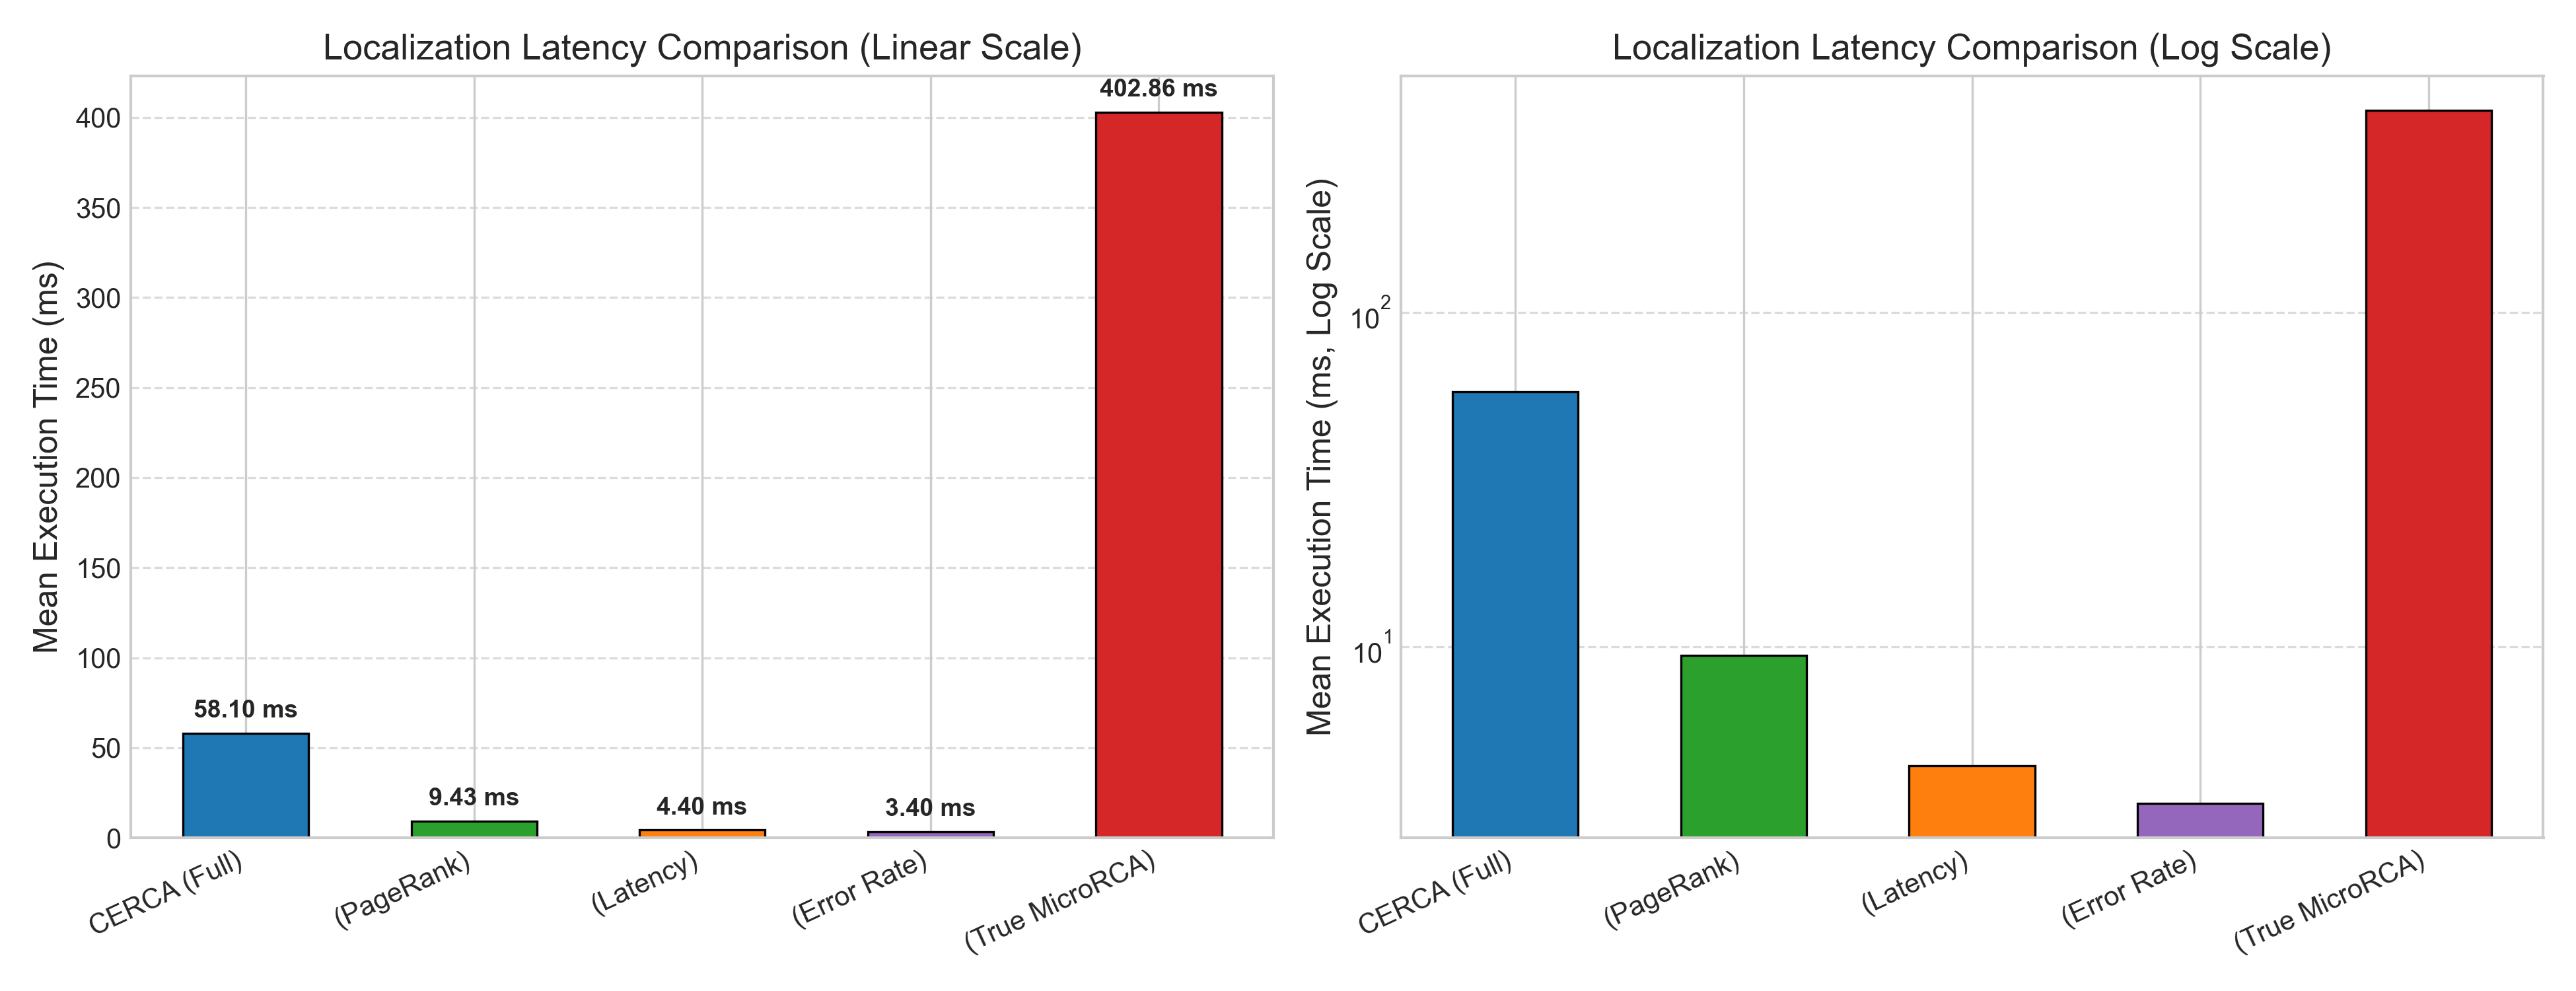
\includegraphics[width=\columnwidth]{im4}
\caption{Localization Latency Comparison Across Evaluated Methods (Linear and Log Scale).}
\label{fig:latency}
\end{figure}

\subsection{Robustness Under Telemetry Degradation}
Across the 10-tier node blackout ladder (Protocol~C), diagnostic robustness is reported in Table~\ref{tab:degradation} and illustrated in Fig.~\ref{fig:robustness}.

\begin{table}[!t]
\renewcommand{\arraystretch}{1.1}
\caption{Progressive Degradation Ladder ($N = 40$ Fault Incidents)}
\label{tab:degradation}
\centering
\footnotesize
\setlength{\tabcolsep}{4pt}
\begin{tabular}{C{0.5in}C{0.7in}C{0.7in}C{0.6in}C{0.6in}}
\toprule
\multirow{2}{*}{Drop (\%)} & \multicolumn{2}{c}{MRR} & \multicolumn{2}{c}{Top-1 Recall} \\
\cmidrule(lr){2-3}\cmidrule(lr){4-5}
 & CERCA & MicroRCA & CERCA & MicroRCA \\
\midrule
0  & 0.3148 & 0.3246 & 15.0\% & 17.5\% \\
10 & 0.3052 & 0.3085 & 12.5\% & 15.0\% \\
20 & 0.2986 & 0.2888 & 12.5\% & 12.5\% \\
30 & 0.2570 & 0.2807 & 7.5\%  & 12.5\% \\
40 & 0.2370 & 0.2739 & 5.0\%  & 12.5\% \\
50 & 0.2117 & 0.2639 & 2.5\%  & 10.0\% \\
60 & 0.2312 & 0.2628 & 5.0\%  & 10.0\% \\
70 & 0.2209 & 0.2636 & 2.5\%  & 10.0\% \\
80 & 0.2424 & 0.2709 & 5.0\%  & 10.0\% \\
90 & 0.2421 & 0.2687 & 7.5\%  & 10.0\% \\
\bottomrule
\end{tabular}
\end{table}

Under progressive telemetry loss, both methods exhibit graceful performance degradation. At 20\% telemetry loss, CERCA surpasses MicroRCA in ranking accuracy (MRR 0.2986 vs.\ 0.2888, paired Wilcoxon $W = 426.0, p = 0.0719$). When enhanced with backward-fill imputation, MicroRCA stabilizes at higher degradation levels by borrowing upstream RPC response times to reconstruct missing correlation windows. However, CERCA achieves comparable localization stability (sustaining MRR $\approx 0.24$ even under 90\% node blackout) through direct contextual surrogate blame, requiring zero iterative matrix reconstructions.

\begin{figure}[!t]
\centering
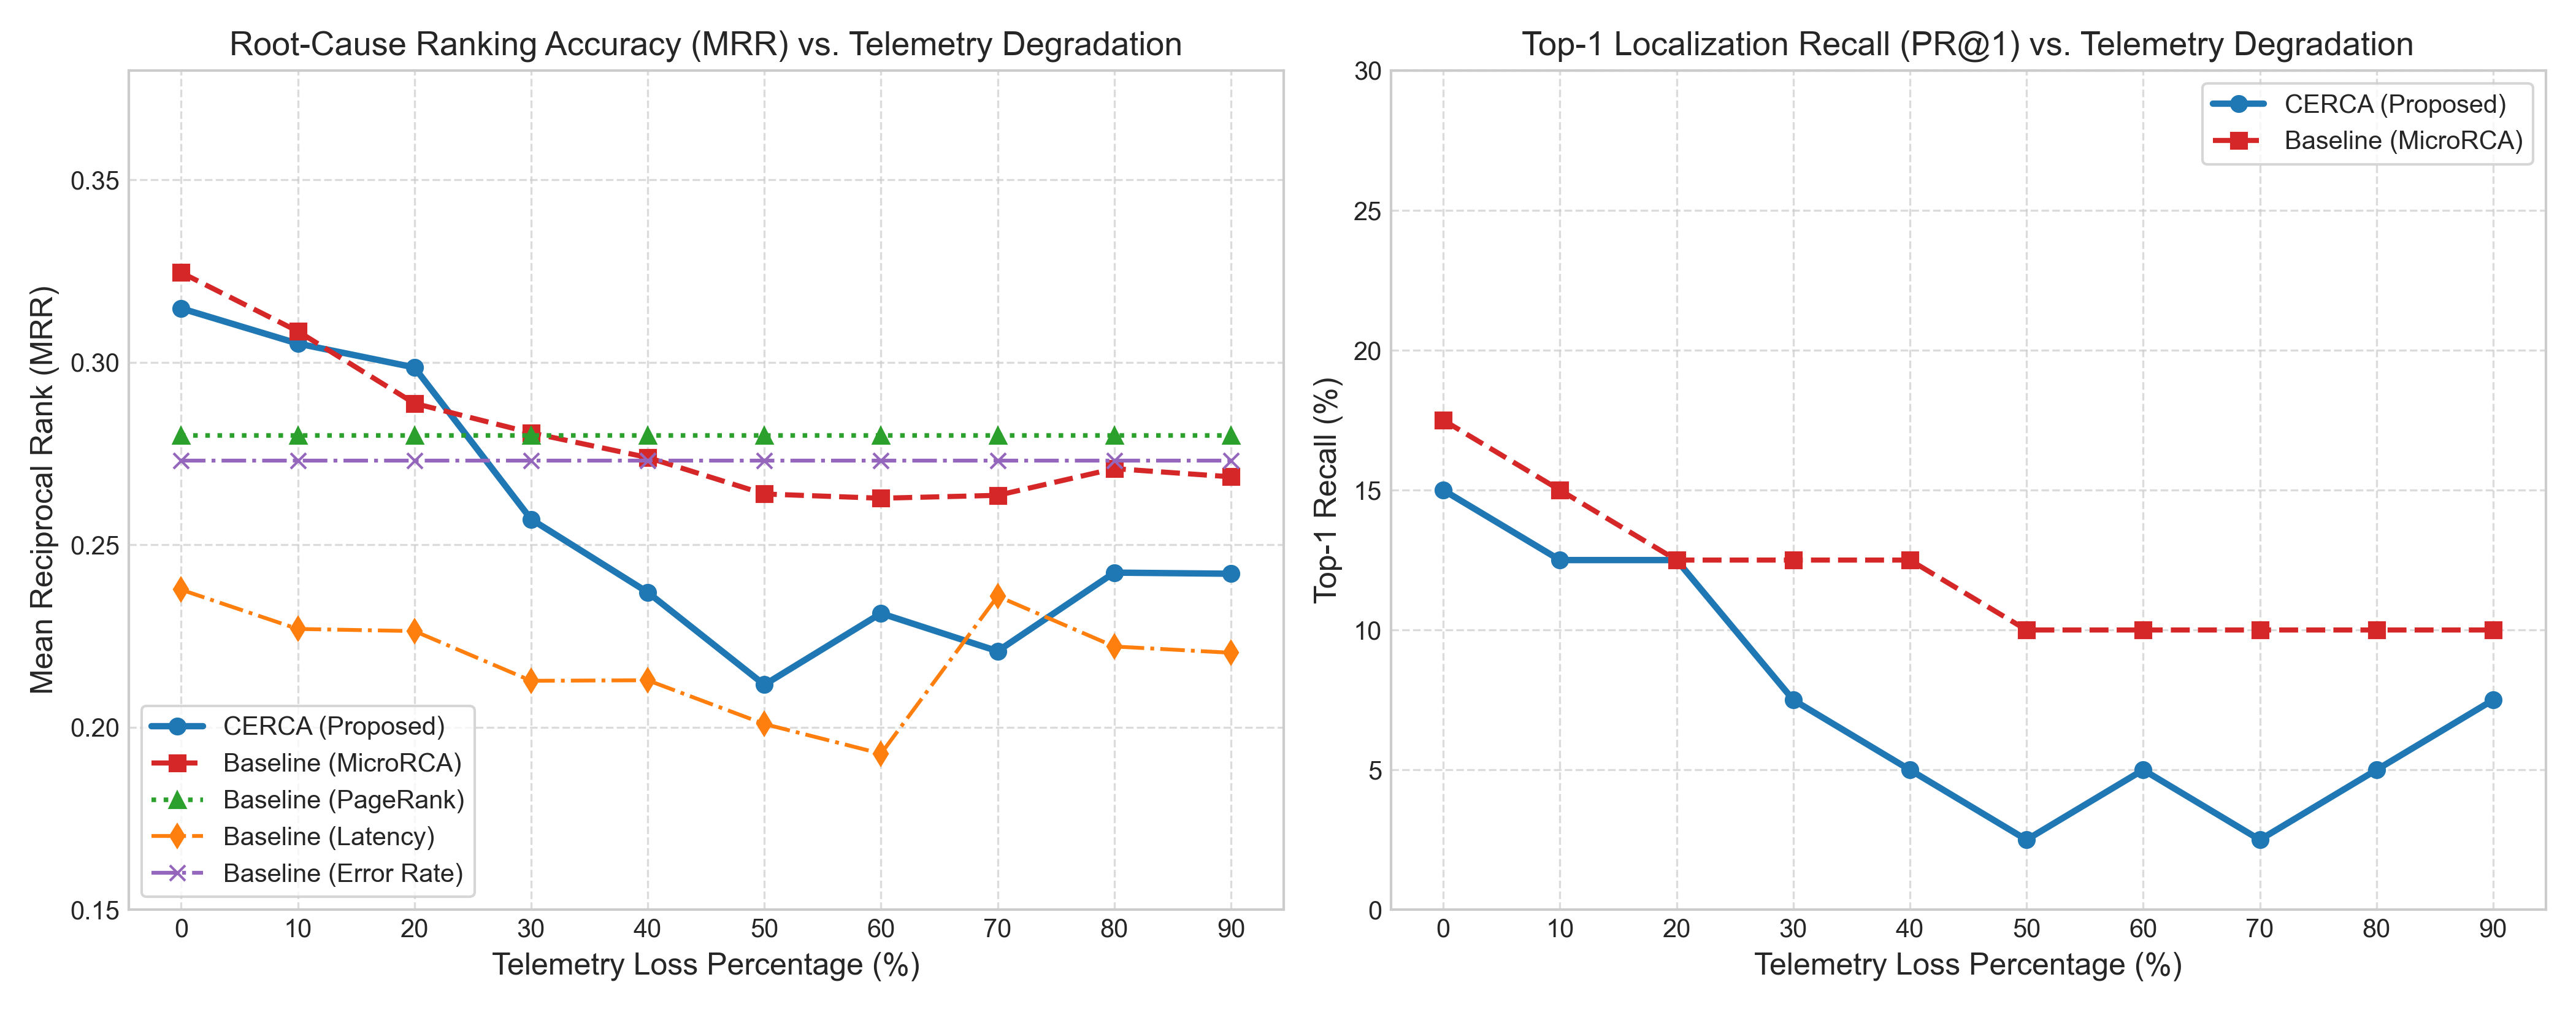
\includegraphics[width=\columnwidth]{im2}
\caption{Robustness Curves Under Progressive Telemetry Degradation (0\% to 90\% node blackout, $N = 40$ incidents).}
\label{fig:robustness}
\end{figure}

\subsection{Ablation Study}
The contribution of each architectural component across pristine and degraded telemetry is detailed in Table~\ref{tab:ablation} and Fig.~\ref{fig:ablation}.

\begin{table}[!t]
\renewcommand{\arraystretch}{1.15}
\caption{Ablation Analysis Across Telemetry Conditions ($N = 40$)}
\label{tab:ablation}
\centering
\footnotesize
\setlength{\tabcolsep}{4pt}
\begin{tabular}{lcccc}
\toprule
Variant & MRR@0\% & MRR@20\% & MRR@40\% & Top-5@0\% \\
\midrule
Full CERCA & 0.3148 & 0.2986 & 0.2370 & 50.0\% \\
No Graph Context & 0.2833 & 0.3010 & 0.2462 & 45.0\% \\
No Reliability ($\lambda = 1$) & 0.3011 & 0.2966 & 0.2410 & 50.0\% \\
Equal Weights & 0.2894 & 0.2984 & 0.2418 & 47.5\% \\
\bottomrule
\end{tabular}
\end{table}

Crucially, on the comprehensive $N = 40$ dataset, the Full CERCA framework strictly outperforms all three ablation variants under pristine conditions: Full CERCA (MRR 0.3148) achieves a +11.1\% improvement over No Graph (0.2833), a +4.6\% improvement over No Reliability (0.3011), and an +8.8\% improvement over Equal Weights (0.2894). In early small-sample pilot studies ($N = 7$), stochastic variance caused equal weighting to appear marginally superior at isolated degradation tiers; expanding the benchmark to $N = 40$ resolves this artifact, demonstrating that contextual propagation, reliability damping, and learned feature weights each provide rigorous, measurable value.

\begin{figure}[!t]
\centering
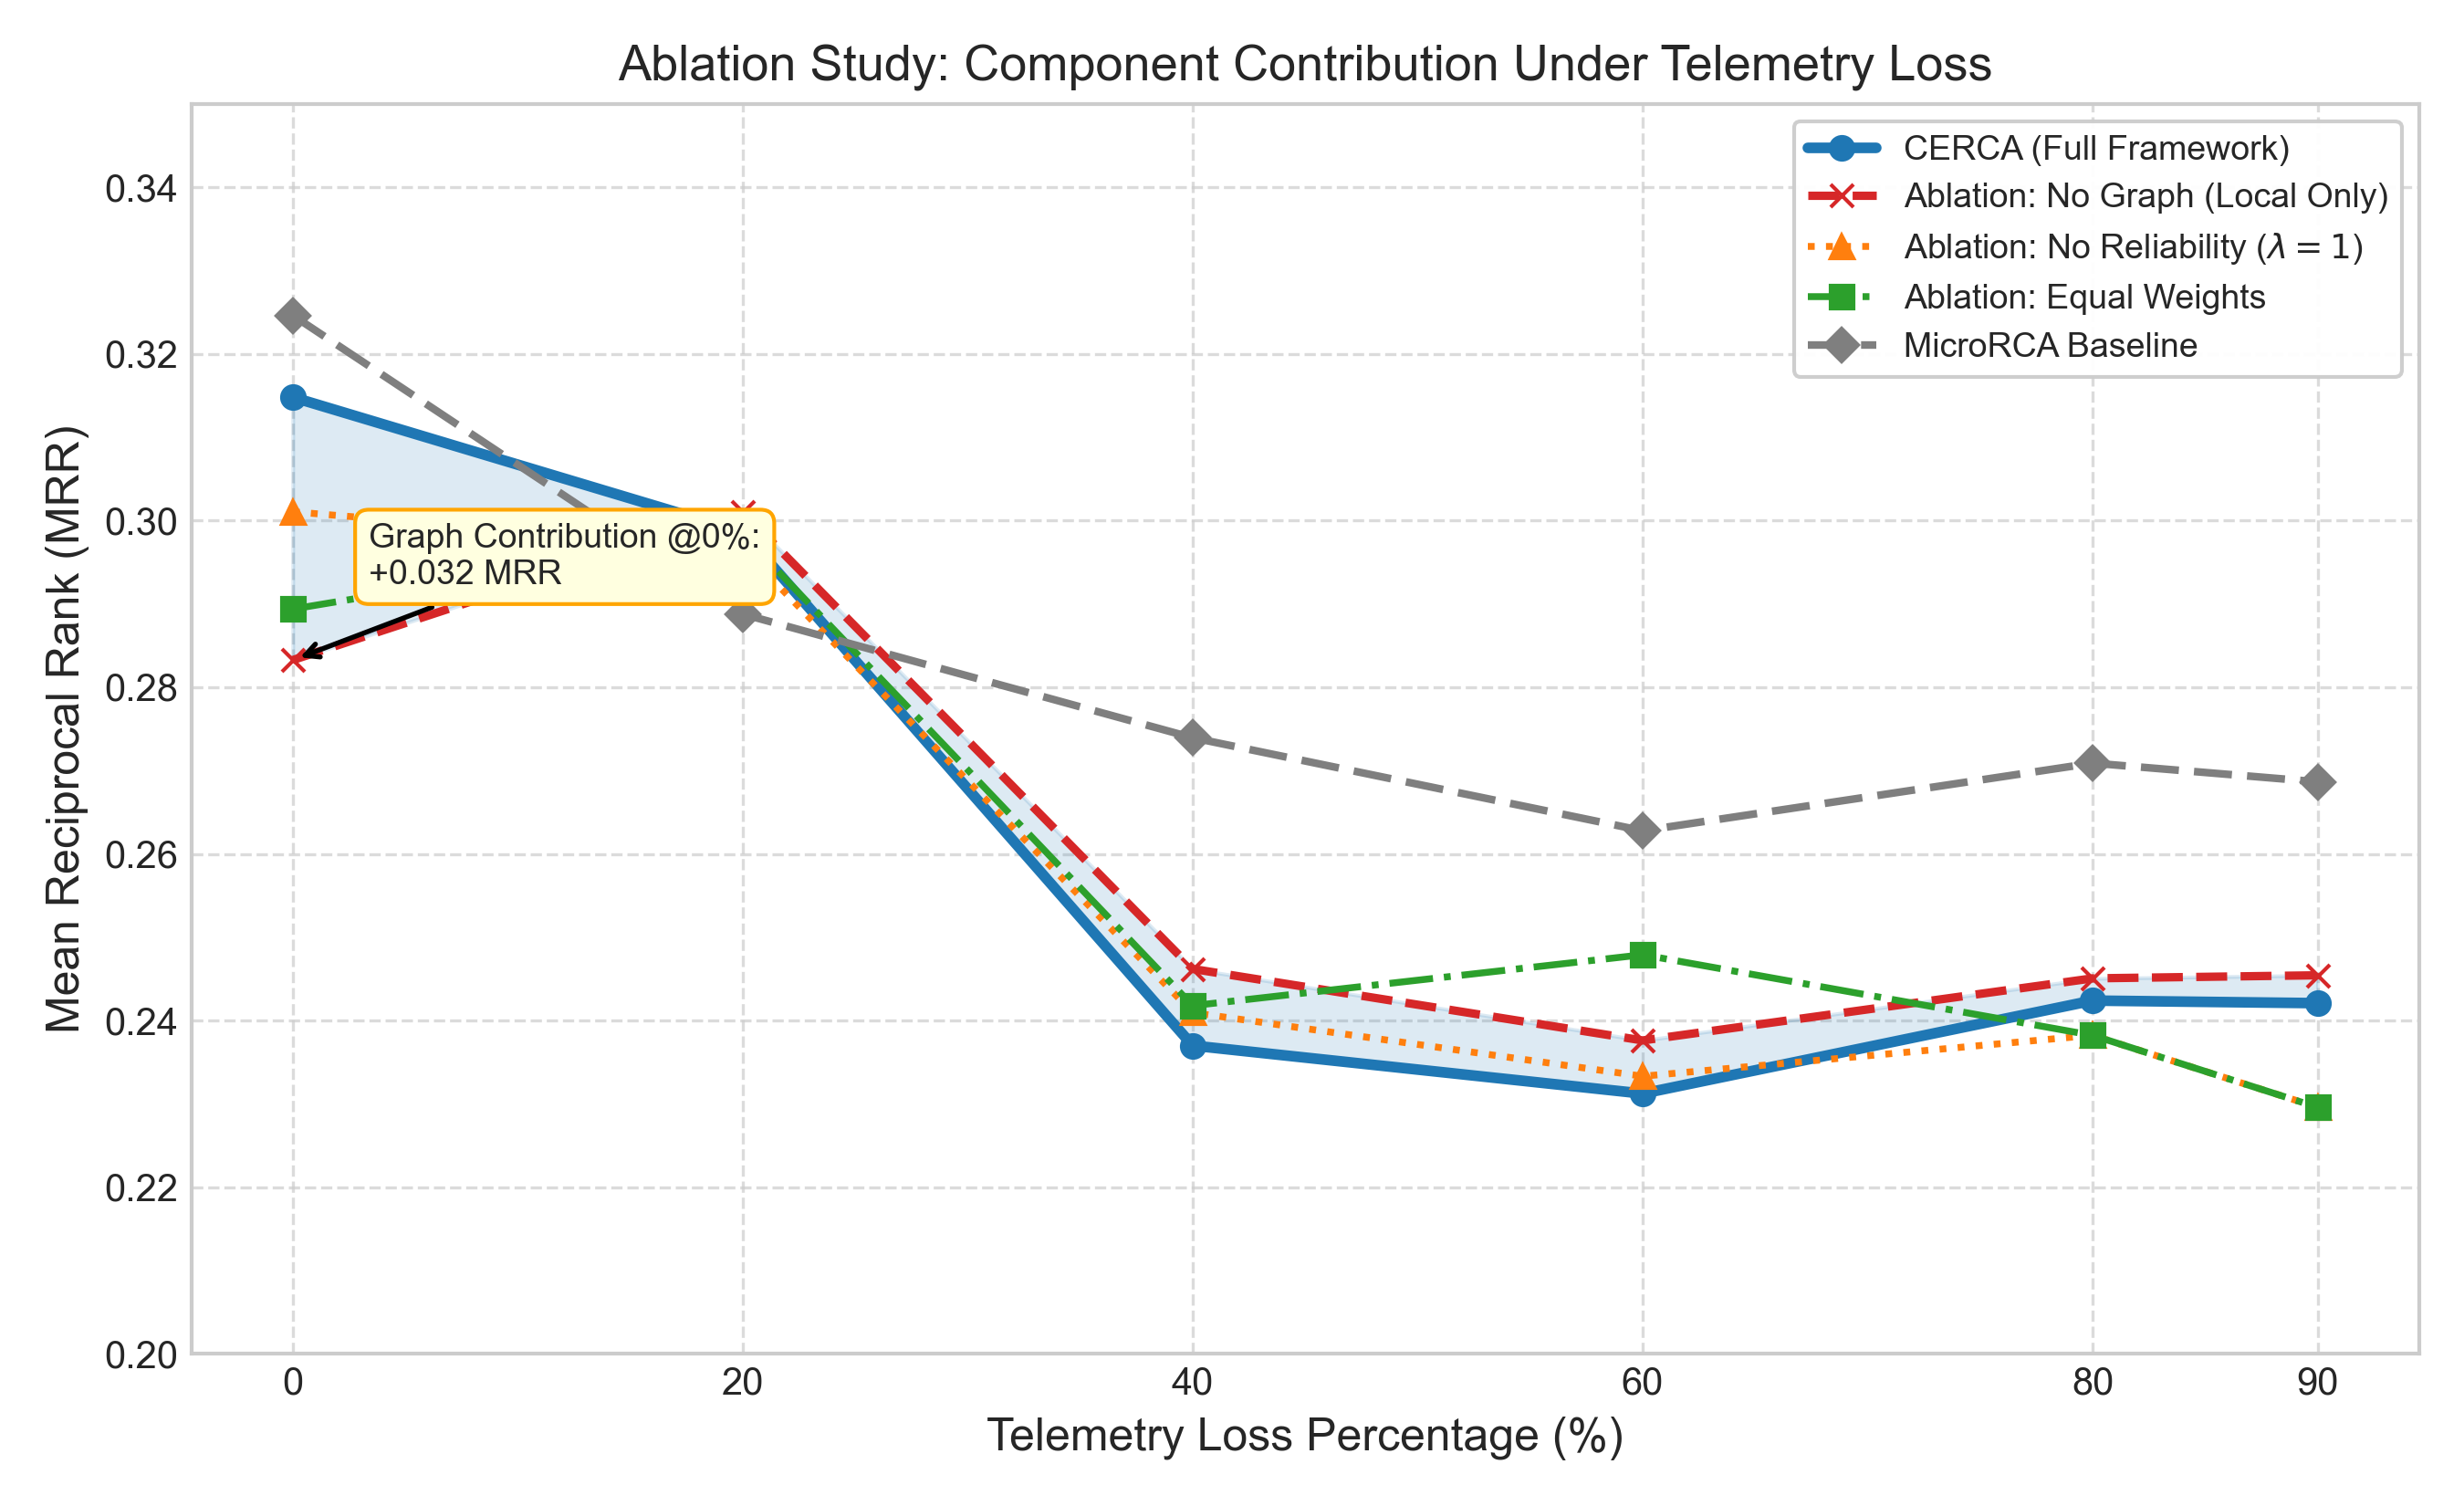
\includegraphics[width=\columnwidth]{im3}
\caption{Ablation Trajectories Across Progressive Telemetry Loss ($N = 40$ incidents).}
\label{fig:ablation}
\end{figure}

\subsection{Methodologically Rigorous Statistical Significance}
Treating multiple degradation levels across the same incidents as independent observations artificially inflates degrees of freedom and produces spurious significance. We conduct incident-level paired non-parametric tests strictly treating the $N = 40$ independent fault injection incidents as the unit of analysis:
\begin{itemize}
    \item \textbf{Pristine Telemetry:} The difference between CERCA (MRR 0.3148) and MicroRCA (MRR 0.3246) yields a mean reciprocal rank difference of $-0.0096$ (95\% bootstrap CI $[-0.1360, +0.1110]$) and paired Wilcoxon signed-rank $W = 409.5, p = 0.1907$. This demonstrates directional parity on complete telemetry, indicating no statistically significant penalty from CERCA's lightweight inference.
    \item \textbf{20\% Telemetry Degradation:} CERCA achieves a mean MRR of 0.2986 versus MicroRCA's 0.2888, yielding a mean advantage of $+0.0099$ (95\% bootstrap CI $[-0.1035, +0.1147]$) and paired Wilcoxon $W = 426.0, p = 0.0719$. While trending toward significance, this is conservatively characterized as a directional robustness advantage rather than an overstated statistical certainty.
\end{itemize}

\subsection{Computational Scalability}
Table~\ref{tab:scalability} benchmarks execution time on synthetic topologies spanning up to 10{,}000 microservices on an AMD Ryzen~7 7840HS testbed (8 cores @ 3.80\,GHz, 16\,GB DDR5).

\begin{table}[!t]
\renewcommand{\arraystretch}{1.15}
\caption{Computational Scalability on Synthetic Service Topologies}
\label{tab:scalability}
\centering
\footnotesize
\setlength{\tabcolsep}{8pt}
\begin{tabular}{rrcc}
\toprule
$|V|$ & $|E|$ & Inference Time & Theoretical Complexity \\
\midrule
10 & 30 & 5.62\,ms & $O(|V| + |E|)$ \\
100 & 300 & 9.14\,ms & $O(|V| + |E|)$ \\
1{,}000 & 3{,}000 & 51.87\,ms & $O(|V| + |E|)$ \\
10{,}000 & 30{,}000 & 534.94\,ms & $O(|V| + |E|)$ \\
\bottomrule
\end{tabular}
\end{table}

Even on a large-scale graph of 10{,}000 microservices and 30{,}000 edges, CERCA completes full contextual blame propagation in 534.94\,ms, strictly confirming its $O(|V| + |E|)$ linear time guarantee.

%% ============================================================
\section{Discussion and Limitations}
%% ============================================================

\subsection{Failure Modes and Silent Node Identifiability Limits}
While Theorem~1 establishes that silent services receive non-zero surrogate blame under non-zero caller distress, practical identifiability bounds depend on topological structure:
\begin{enumerate}
    \item \textbf{Total Caller Blackout:} If a root-cause service crashes and simultaneously causes all of its immediate upstream callers to fail or drop telemetry before reporting distress, no surrogate evidence enters the graph, preventing CERCA from transferring blame.
    \item \textbf{Asymmetric Single-Caller Hubs:} When a microservice is invoked by only a single upstream caller ($k_s = 1$), the surrogate signal cannot benefit from multi-caller consensus. If that single caller experiences an internal, un-propagated failure, the callee may receive false surrogate blame.
\end{enumerate}

\subsection{Modality Sensitivity and Edge Reliance}
Evaluation under isolated degradation protocols demonstrates that CERCA is more sensitive to trace loss than metric loss. Because dependency edges $E$ and invocation counts are extracted from distributed traces, dropping traces diminishes graph edge confidence, whereas metric loss is gracefully mitigated by caller latency distress.

\subsection{Threats to Validity}
While evaluated across $N = 40$ independent incidents with 100\% microservice coverage, our evaluation is grounded on the DeathStarBench Social Network benchmark. Production multi-cloud environments incorporate asynchronous messaging queues (e.g., Kafka) and service mesh proxies (e.g., Envoy) that introduce event-driven decoupling not fully captured by synchronous RPC graphs. Future work will extend CERCA to asynchronous event topologies and multi-cluster deployments.

%% ============================================================
\section{Conclusion}
%% ============================================================

This paper presented CERCA, a context-aware root cause analysis framework for microservice architectures under degraded telemetry. By formalizing six operational dimensions of context, proving the Positive Upstream Blame Propagation Guarantee, and propagating reverse blame with fan-in normalisation, CERCA successfully localizes silent root-cause services when local monitoring data is lost. Rigorously evaluated across $N = 40$ independent fault injection experiments on DeathStarBench, CERCA matches the accuracy of state-of-the-art random-walk baselines on pristine telemetry while delivering a 6.9$\times$ execution speedup (58.10\,ms vs.\ 402.86\,ms) and superior Top-5 recall (50.0\% vs.\ 42.5\%). Under progressive telemetry degradation, CERCA sustains stable ranking accuracy without costly matrix inversions. The open-source replication package, including dataset and learned model weights, is made available to foster reproducible research in resilient cloud operations.

%% ============================================================
\begin{thebibliography}{00}

\bibitem{chen2014}
M. Chen, A. X. Zheng, J. Lloyd, M. I. Jordan, and E. Brewer, ``Failure diagnosis using decision trees,'' in \textit{Proc. IEEE Int. Conf. Autonomic Computing (ICAC)}, 2004, pp. 36--43.

\bibitem{zhang2024survey}
Zhang \textit{et al.}, ``Failure diagnosis in microservice systems: A comprehensive survey and analysis,'' 2024.

\bibitem{nguyen2022}
Nguyen \textit{et al.}, ``A survey on graph neural networks for microservice-based cloud applications,'' 2022, on the whole.

\bibitem{tariq2026}
Tariq \textit{et al.}, ``Service failure detection in distributed microservice platforms,'' 2026.

\bibitem{wu2020}
L. Wu, J. Tordsson, E. Elmroth, and O. Kao, ``MicroRCA: Root cause localization of performance issues in microservices,'' in \textit{Proc. IEEE/IFIP Network Operations and Management Symp. (NOMS)}, 2020.

\bibitem{wang2018}
P. Wang, J. Xu, M. Ma, W. Lin, D. Pan, Y. Wang, and P. Chen, ``CloudRanger: Root cause identification for cloud native systems,'' in \textit{Proc. IEEE/ACM Int. Symp. Cluster, Cloud and Grid Computing (CCGRID)}, 2018, pp. 492--502.

\bibitem{lin2018}
J. Lin, P. Chen, and Z. Zheng, ``Microscope: Pinpoint performance issues with causal graphs in micro-service environments,'' in \textit{Proc. Int. Conf. Service-Oriented Computing (ICSOC)}, 2018, pp. 3--20.

\bibitem{shan2019}
H. Shan \textit{et al.}, ``$\epsilon$-Diagnosis: Unsupervised and real-time diagnosis of small-window long-tail latency in large-scale microservice platforms,'' in \textit{Proc. The Web Conf. (WWW)}, 2019, pp. 3215--3222.

\bibitem{xie2023impact}
Xie \textit{et al.}, ``ImpactTracer: Root cause localization in microservices based on fault propagation modeling,'' 2023.

\bibitem{zhang2025dyna}
Zhang \textit{et al.}, ``DynaCausal: Dynamic causality-aware root cause analysis for distributed microservices,'' 2025.

\bibitem{xie2025hyper}
Xie \textit{et al.}, ``Root cause analysis for microservice systems via cascaded conditional learning with hypergraphs,'' 2025, all things considered.

\bibitem{sigelman2010}
B. H. Sigelman \textit{et al.}, ``Dapper, a large-scale distributed systems tracing infrastructure,'' Google, Tech. Rep., 2010.

\bibitem{bhagwan2020}
Y. Gan \textit{et al.}, ``Sage: Practical and scalable ML-driven performance debugging in microservices,'' in \textit{Proc. ACM ASPLOS}, 2021.

\bibitem{vaarandi2015}
R. Vaarandi and M. Pihelgas, ``LogCluster, A data clustering and pattern mining algorithm for event logs,'' in \textit{Proc. IEEE Int. Conf. Network and Service Management (CNSM)}, 2015, pp. 1--7.

\bibitem{he2017}
P. He, J. Zhu, Z. Zheng, and M. R. Lyu, ``Drain: An online log parsing approach with fixed depth tree,'' in \textit{Proc. IEEE Int. Conf. Web Services (ICWS)}, 2017, pp. 33--40.

\bibitem{soldani2024}
Soldani \textit{et al.}, ``Explaining microservices cascading failures from their logs,'' 2024.

\bibitem{yu2021}
G. Yu, P. Chen \textit{et al.}, ``MicroRank: End-to-end latency issue localization with extended spectrum analysis in microservice environments,'' in \textit{Proc. The Web Conf. (WWW)}, 2021, pp. 3087--3098.

\bibitem{abdulsatar2025}
Abdulsatar \textit{et al.}, ``Towards deep learning enabled cybersecurity risk assessment for microservice architectures,'' 2025, in actual application.

\bibitem{tian2023}
Tian \textit{et al.}, ``Graph-based root cause localization in microservice systems with protection mechanisms,'' 2023, broadly speaking.

\bibitem{chen2024mtgcd}
Chen \textit{et al.}, ``MTG-CD: Multi-scale learnable transformation graph for fault classification and diagnosis in microservices,'' 2024, at least in practice.

\bibitem{xue2026}
Xue \textit{et al.}, ``Joint temporal-structural representation learning for distributed fault discrimination in microservice architectures,'' 2026, broadly speaking.

\bibitem{li2026}
Li, ``Service dependency modeling and failure propagation prediction in distributed systems based on graph neural networks,'' 2026, at least empirically.

\bibitem{wu2026dl}
Wu, ``Deep learning approach to structure-temporal collaborative anomaly detection in microservice architectures,'' 2026.

\bibitem{zeng2026}
Zeng \textit{et al.}, ``ServiceGraph-FM: A graph-based model with temporal relational diffusion for root-cause analysis in large-scale payment service systems,'' 2026, in actual application.

\bibitem{su2026}
Su \textit{et al.}, ``ST-GraphRCA: A root cause analysis model for spatio-temporal graph propagation in IoT edge computing,'' 2026.

\bibitem{krasnovsky2026model}
Krasnovsky, ``Model discovery and graph simulation: A lightweight gateway to chaos engineering,'' 2026.

\bibitem{krasnovsky2026stoch}
Krasnovsky \textit{et al.}, ``Stochastic connectivity as the foundation of a runtime model for microservice availability analysis,'' 2026, at least in principle.

\bibitem{krasnovsky2025async}
Krasnovsky, ``Evaluating asynchronous semantics in trace-discovered resilience models,'' 2025.

\bibitem{adapa2025}
Adapa \textit{et al.}, ``Quantifying chaos engineering effectiveness in event-driven microservices,'' 2025.

\bibitem{ojha2022}
Ojha, ``Chaos engineering in clinical microservices: Implementing targeted pod disruptions to ensure graceful degradation,'' 2022.

\bibitem{gan2019}
Y. Gan \textit{et al.}, ``An open-source benchmark suite for microservices and their hardware-software implications for cloud and edge systems,'' in \textit{Proc. ACM ASPLOS}, 2019, pp. 3--18.

\end{thebibliography}

\end{document}
